 \section{Literature Review and State of the Art Analysis}

This chapter discusses the fundamentals of motion planning and related concepts. According to \cite{1} Motion planning consists of the following basic concepts which are prevalent irrespective of the type of planning problem:
\begin{itemize}
\item A \textbf{state space} definition in which the all probable scenarios related to the planning problem can be expressed
\item Modeling \textbf{time} respective to the problem, which can determine the speed of the execution of the problem or the order of sequence in which certain actions should be completed.
\item \textbf{Actions} are generated by plans which manipulate a state. The relationship between an an action and state change is generally described by the user. 
\item \textbf{Initial and Goal States} are the defined by the user. Actions are generated in order to convert the initial state to goal state.
\item Usually a \textbf{criterion} is specified in order to execute the actions to have a desired outcome. The two main goals of specifying a criterion are:
\begin{enumerate}
\item \textbf{Feasibility} The goal state can be reached 
\item \textbf{Optimality} Optimizes the performance of the planner e.g. reducing the planning time, taking actions with low cost, while achieving the goal state 
\end{enumerate}
\item \textbf{Plan} is generally a sequence of actions which might be simple or complex depending on the above mentioned criteria. 
\end{itemize}
In the following sections we delve deeper into motion planning for a manipulator 


\subsection{Motion Planning for Industrial Manipulators}
Motion planning is one of the most important aspects, when it comes to efficient program generation for industrial robots. Efficient motion planning can not only reduce time of task execution but also increase the rate of task completion by ensuring pitfalls of collision or singular points are avoided. For industrial manipulators generated plans need to be highly accurate and precise, hence large factories, namely automobile manufacturers employ robots which are pre programmed. However when it comes to small and medium enterprises, where the key goal is to adapt the manufacturing process based on the task at hand, hard coding a robot is not desirable. A very good example of this is welding, where the task changes based on the workpiece to be welded. Workpieces can be of varying complex geometrical structures and the multiple joints may need to welded at each iteration. Hence to maintain the same level of efficiency and speed of execution it becomes necessary to generate optimal motion plans.  

\subsubsection{Motion Planning for multi-DoF manipulators}

This section will highlight various existing motion planning approaches and discuss the pros and cons of each. In \cite{2}(Collision free path planning..) the authors model the state space as a 3D discretized grid in Cartesian coordinate system. The workpiece and fixtures are modeled as collision onjects. A heuristic is introduced which determines the distance between goal and current location while the collision avoidance is handled by a function which calculates the distance between current location and nearest collision objects and assigns a cost value based on the distance,as illustrated with equations \eqref{eq1},\eqref{eq2},\eqref{eq3}
\begin{equation}
\label{eq1}
obs = \sum x_{n} - m:x_{n} + m,y_{n} - m:y_{n} + m:z_{n} - m:z_{n} + m
\end{equation}
\begin{equation}
\label{eq2}
d = \sqrt{(x_{n} - x_{c})^2 + (y_{n} - y_{c})^2 + (z_{n} - z_{c})^2} + k*obs
\end{equation}
\begin{equation}
\label{eq3}
h = \sqrt{(x_{g} - x_{n})^2 + (y_{g} - y_{n})^2 + (z_{g} - z_{n})^2} + d
\end{equation}
here k is a constant [$x_{c},y_{c},z_{c}$] defines the current node, [$x_{n},y_{n},z_{n}$] represents the neighboring node and [$x_{g},y_{g},z_{g}$] defines the goal node. The A* algorithm is used to search the tree generated from this definition. Once a path to the goal state has been found, it is checked for inverse kinematic feasibility. The generated joint values are again checked for collision avoidance and then it is passed to the robot program. The main drawback of this approach is as the search tree tries to generate path which are away from obstacles while the workpiece object is designated as a collision object, which results in the manipulator moving far away from the workpiece after it has finished welding one edge. In cases where only one edge needs to be welded there the result will remain unaffected, however for multi edge welding this approach will lead to unnecessary large path costs. Another highlight of this approach was to reduce time of execution by generating trajectories, but the fact that each time the inverse kinematic values are generated; it is rechecked for collision leads to a delay (as collision checking is a computationally expensive process) and eliminates the gains of the trajectory planning. The fact that the authors did not publish any experimental evaluation of their method in the paper leaves open questions in this regard. \\
In \cite{3}(Online minimum time trajectory planning), the authors propose an algorithm for computing the trajectory of a 6 DoF manipulator which is explained with the help of the following flowchart. The equation \eqref{eq4} for calculating the maximum allowable acceleration and deceleration is 
\begin{equation}
\label{eq4}
\ddot{p}_{max} = \lambda_{min}u_{\ddot{p}}\in \Re^{m}
\end{equation}
where p is the maximum acceleration in cartesian space.

\begin{figure}[htbp] %  figure placement: here, top, bottom, or page
 \centering
   %\includegraphics[angle=90,width=10cm]{images/tbox.jpg}
   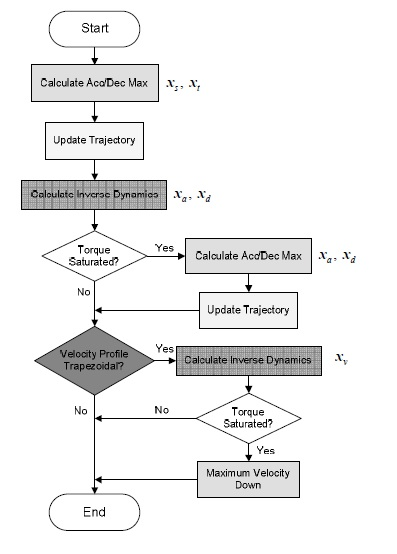
\includegraphics[width=9cm]{images/AlgoFlowchart.jpg}
   \caption[Trajectory Algorithm]
   {Trajectory Algorithm \footnotemark[\value{footnote}]}
   
\label{fig:img1}
\end{figure}

In \cite{4}(Integrated Time Optimal Trajectory Planning), the authors propose an algorithm to ensure compliance of the robot motion path and the planned path at high speeds. The authors demonstrate the working of their algorithm using a parameterized circular path using the equation \eqref{eq5}
\begin{equation}
\label{eq5}
q= \begin{bmatrix} q_{1}^{*}(t)\\ q_{2}^{*}(t)\\ q_{3}^{*}(t) \end{bmatrix} = \phi (\theta)|_{\theta=\theta^{*}(t)} = \begin{bmatrix} \phi_{1}(\theta)\\ \phi_{2}(\theta)\\ \phi_{3}(\theta) \end{bmatrix}|_{\theta=\theta^{*}(t)}
\end{equation}
In this equation the time parameterization is replaced by [$\theta$] parameterization which results in a synchronization of joints. Due to this joint velocities can be assigned with the following equation \eqref{eq6} for any velocity profile
\begin{equation}
\label{eq6}
q=\phi^{'}(\theta)\dot{\theta}
\end{equation}
After finding the optimal joint velocities, the joint angles are checked whether they satisfy the dynamic constraints. The authors then implemented an Proportional Derivative(PD) control feedback loop as a supplement to the motion planner. The authors propose their own controller apart from the already implemented PD controller and showed that their implementation lead to faster convergence to desired trajectory. The key takeaway from this paper is the parameterized model of trajectory planning which ensures the joint values can be assigned with variables dependent on angle value- [$\theta$] instead of time. 
\subsubsection{Motion Planning for manipulator and rotary table systems}
A key requirement for producing highest quality weld is the \textbf{downhand} welding position, in which the tangent line to the weld is horizontal and the normal vector to the weld is vertical \cite{5}(Manufacturing Process Planning for Robotic Arc-Welding Station). Due to this fixed criteria, planned paths for welding often end up having singular points in them, or they encounter collision objects which are difficult to avoid without violating the \textbf{downhand} welding position. One of the approaches taken in this regard is to include a till-roll workpiece manipulator or rotary table. In this paper \cite{5} the authors propose a cluster level operation planning with the optimization objective being - minimization of manufacturing time. \\
The authors divide the welding task into several clusters using a technique called weld seam clustering which arranges the welds into groups that do not require altering positioner configuration. The idea is to find the most optimum path through these clusters. The authors use a generalized TSP (GTSP) algorithm with GI3 heuristics which incorporates the following 3 phases (i) Generalized Initialization, (ii) Generalized Insertion , and (iii) Generalized Improvement. The above mentioned method was able to generate valid optimized solutions for 70-80$\%$ cases with a maximum optimization of 2.6$\%$. A possible reason for this method not generating valid solutions 100$\%$ of the time is due to the fact that, generated solutions are not subjected to kinematic constraints and only to the abstract space constraints like collision avoidance and seam selection checking.





\subsection{Robotic Welding Processes}
In a recent study conducted by the American Welding Association revealed that the current demand for manufacturing welded goods are from small or medium batch manufacturing. In these settings robotic welding provides the most cost effective solution compared to human welders or hard automated setups. In this section we will discuss the various welding methodologies that are compatible with robotic welding and describe them briefly.\\
In \cite{6}(Welding Robots: Technology, System Issues and Application, Pires, J.N. and Loureiro,
A. and Bolmsjo, G), the authors state that the most prevalent method of welding in industry is the arc welding method. The two main types of arc welding are gas shielded tungsten arc welding (GTAW) and the gas shielded metal arc welding (GMAW). Apart from these, the various other methods of welding include Laser Beam Welding(LBW),Resistance Spot Welding (RSW), Friction Stir Welding (FSW).
Since GTAW and GMAW are the welding methods used for robotic welding in industries, we will elaborate on these.
\begin{itemize}
\item \textit{GTAW}: In this process an arc is created between a non-consumable electrode and the work metal which is then shielded by an inert gas to remove any atmospheric contamination. A current of 50-700 A is used to melt and fuse the work metal.
\item \textit{GMAW}: In this process a consumable electrode is used. A high current is applied which melts both the electrode and the work metal and fuses them together. An inert gas is used here as well to prevent contamination. The magnitude of current and voltage, size of electrode and type of inert gas used, determines the type of welding method:spray, short-circuiting, globular and pulsed transfer.
\end{itemize}

\subsubsection{Analysis of existing methods of Robtic Welding}
\textbf{Gas Tungsten Arc Welding (GTAW):}
\begin{figure}[htbp] %  figure placement: here, top, bottom, or page
 \centering
   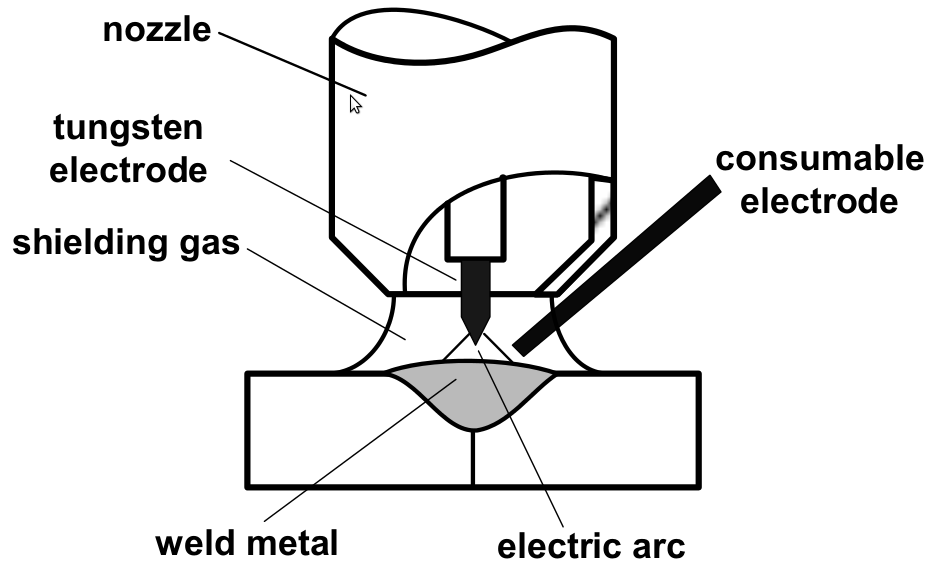
\includegraphics[width=9cm]{images/GTAW.png}
   \caption[Gas Tungsten Arc Welding]
   {Gas Tungsten Arc Welding \footnotemark[\value{footnote}]}  
\label{fig:img2}
\end{figure}
\newpage
\textbf{Gas shielded metal arc welding (GMAW):}

\begin{figure}[htbp] %  figure placement: here, top, bottom, or page
 \centering
   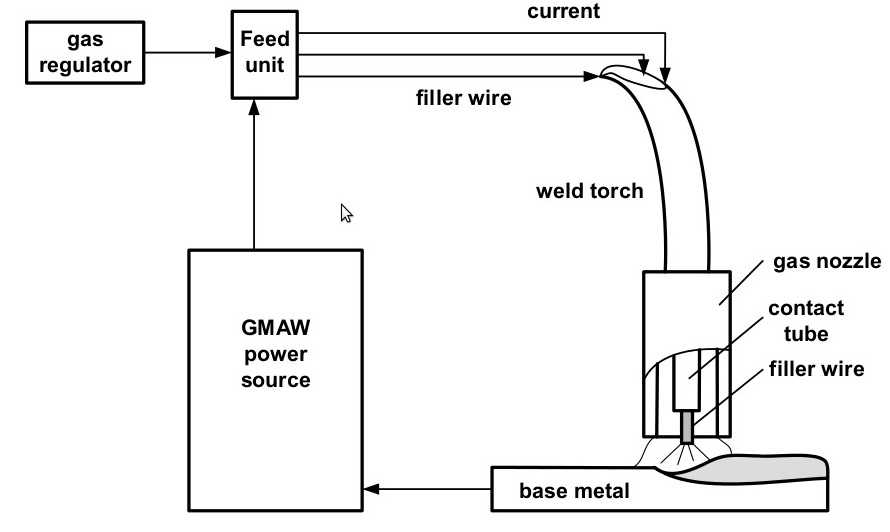
\includegraphics[width=9cm]{images/GMAW.png}
   \caption[Gas Metal Arc Welding]
   {Gas Metal Arc Welding \footnotemark[\value{footnote}]}  
\label{fig:img3}
\end{figure}

\begin{table}[]
\centering
\caption{Comparison of GMAW and GTAW welding}
\label{my-label}
\begin{tabular}{|c|c|c|}
\hline
                       & \textbf{GMAW}                                                                                                                                                  & \textbf{GTAW}                                                                                         \\ \hline
Power Sources          & Constant voltage type                                                                                                                                          & Constant current type                                                                                 \\ \hline
Electrodes             & Consumable type                                                                                                                                                & Non-consumable type                                                                                   \\ \hline
Current                & \begin{tabular}[c]{@{}c@{}}Direct current electrode positive\\  applied to weld head\end{tabular}                                                              & \begin{tabular}[c]{@{}c@{}}Direct current electrode negative\\ applied to weld head\end{tabular}      \\ \hline
Welding Speed          & \begin{tabular}[c]{@{}c@{}}A small increase in speed leads to \\ greater weld material penetration \\ but beyond a threshold leads to \\ undercut\end{tabular} & \begin{tabular}[c]{@{}c@{}}Changing welding speed \\ has no effect on quality of \\ weld\end{tabular} \\ \hline
Arc Length             & between 5-15mm                                                                                                                                                 & usually 2-5mm                                                                                         \\ \hline
Electrode Vertex angle & \begin{tabular}[c]{@{}c@{}}Usually kept at 45$\deg$ to normal\\  of the weld edge\end{tabular}                                                                & \begin{tabular}[c]{@{}c@{}}Angles between 30$\deg$ -\\ 120$\deg$\end{tabular}                       \\ \hline
\end{tabular}
\end{table}

\subsection{Multi Robot Approaches for Welding}

One of the major drawbacks of robotic welding is the inability of the welding robot to manipulate the object. While for simple tasks, this does not pose a challenge, however for welding complex work pieces or for avoiding collision in the welding path, it becomes necessary to manipulate the object as well. In this section we will illustrate some of the well known and used approaches for multi robot welding. 
A well used approach to address this problem, is using two robots instead of one. A 6 dof manipulator is coupled with either a 2 dof rotary table or another 6 dof manipulator. It goes without saying that generating plans for more than one robot is a tedious task all the while maintaining the kinematic and dynamic constraints, as well as following the process parameters. In the next two subsections we will discuss about two popular multi robot planning and control approaches.

\subsubsection{Centralized and De-centralized planning}
A key point in designing multi robot planning approach is to generate motion plans centrally from either one robot or to use distributed planning with each robot planning its own path and then combining them to form a final plan. \\
In \cite{8}(Comparison of alternate methods for distributed motion planning of robot) the authors discuss a distributed planning approach based on artificial potential framework. The authors consider a case of planning path for three robots. The kinematic and dynamic model is formulated followed by the constraint relationship formulation as illustrated by \eqref{eq7},\eqref{eq8},\eqref{eq9}
\begin{equation}
\label{eq7}
\dot{q} = v
\end{equation}
\begin{equation}
\label{eq8}
M(q)\ddot{q} + V(q,\dot{q}) + G(q) = E(q)u - A^{T}\lambda
\end{equation}
\begin{equation}
\label{eq9}
M(q) = \begin{bmatrix} [M_{A}]_{2,2} & 0 & 0\\ 0 & [M_{A}]_{2,2}& 0\\ 0 & 0 & [M_{A}]_{2,2} \end{bmatrix},q = \begin{bmatrix} q_{A}\\ q_{B}\\ q_{C} \end{bmatrix}
\end{equation}
where $q=[x_{i} y_{i}]^{T} \epsilon \Re^{2}$
while the constraint equation is given as follows \eqref{eq10}
\begin{equation}
\label{eq10}
C(q) = \begin{bmatrix} (x_{A} - x_{B})^{2} + (y_{A} - y_{B})^{2} - {c_{AB}}^2\\ (x_{B} - x_{C})^{2} + (y_{B} - y_{C})^{2} - {c_{BC}}^2\\ (x_{C} - x_{A})^{2} + (y_{C} - y_{A})^{2} - {c_{CA}}^2 \end{bmatrix} = \begin{bmatrix} 0\\ 0\\ 0 \end{bmatrix}
\end{equation}
The authors then tested this model with independent parameterization and concluded that the projection based approach is robust but computationally expensive and which increases with each additional step. 
In \cite{13}(Kinematic and dynamic analysis of 3 dof..) the authors describe a decentralized multi robot planning approach for general industrial tasks like welding, milling etc. with a 6 dof manipulator and a 3 dof rotary table. The dynamic equation is illustrated in \eqref{eq11}
\begin{equation}
\label{eq11}
M_{OK} = P_{i}(H_{OK}),H_{OK} = J_{OK}\omega_{i - OK}
\end{equation}
\eqref{eq11} is applied to every point, where each point shown with k symbol has $M_{OK}$ is the external torque, $H_{OK}$ is the rotational momentum and $J_{OK}$ is the moment of inertia for point k and $\omega_{i - OK}$ is the rotational velocity. 
 
\subsubsection{Master Slave Configuration}
One of the major approaches for multi robot planning has been proposed in \cite{7}(kinematic cooperated welding trajectory planning) is master/slave cooperative planning. In this approach an initial kinematic relationship between the frames of the welding seam and the tool tip of the welding robots are established. One of the robots is considered as the master robot and its kinematic chain is defined from the base to its tool tip and for the slave robots the kinematic chain is defined from master robot base to slave robot base to slave robot tool and finally to master robot tool tip. The scheme is illustrated in illustration \ref{fig:img5}.
\begin{figure}[htbp] %  figure placement: here, top, bottom, or page
 \centering
   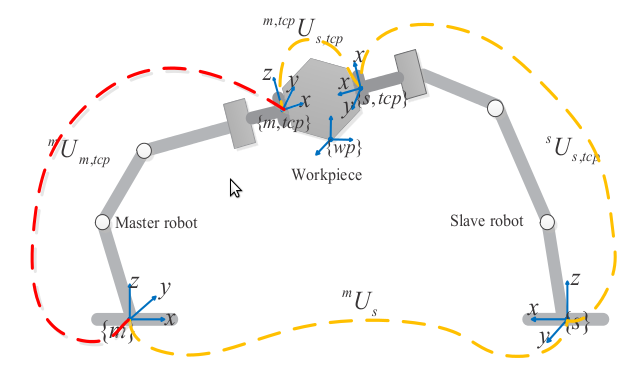
\includegraphics[width=9cm]{images/master_slave_coord.png}
   \caption[Master Slave Coordinate Specification]
   {Master Slave Coordinate Specification \footnotemark[\value{footnote}]}  
\label{fig:img5}
\end{figure}
Master slave configuration can be further divided into tightly coupled master/slave mode and loosely coupled master slave/mode. In tightly coupled master slave mode the master and slave robot assignments are fixed and in lightly coupled system the master slave assignments can be changed. 
The equation for a general master slave configuration is described in \eqref{eq12}, \eqref{eq13} describes a tightly couple master slave configuration and \eqref{eq14} describes the loosely coupled, time based master/slave configuration.
\begin{equation}
\label{eq12}
^{m}U_{m,tcp} = {^{m}U_{s}} \cdot ^{s}U_{s,tcp}\cdot^{s,tcp}U_{m,tcp}
\end{equation}
\begin{equation}
\label{eq13}
^{s}U_{s,tcp}(t) = {^{m}U_{s}}^{-1} \cdot ^{m}U_{m,tcp}(t)\cdot^{m,tcp}U_{s,tcp}
\end{equation}
\begin{equation}
\label{eq14}
^{s}U_{s,tcp}(t) = {^{m}U_{s}}^{-1} \cdot ^{m}U_{m,tcp}(t)\cdot^{m,tcp}U_{s,tcp}(t)
\end{equation}
The authors in \cite{7} then go onto describe three independent scenarios in which master/slave cooperative welding is applied. They are
\begin{enumerate}
\item Plate to plate welding - Welding tool tip of the multiple robots should have consistent relative distance.
\item Tube to plate welding - In this mode of operation, the robot which grips the work piece is considered master robot while the welding robot is configured in slave mode.
\item Tube-tube welding - This mode of operation is similar to tube to plate welding.
\end{enumerate}
Based on the results generated from running experiments for the three use cases, it was concluded that the methods described by the authors, achieve the desired goals successfully, however the actual performance of the methods are not reported. A key aspect of master/slave mode of operation that needs to be kept in mind is, for each welding task an accurate description of the seam to be welded needs to be formulated. For simple seam descriptions, this can be easily achieved, however for complex weld shapes the formulation becomes difficult. A counter approach to this is non-master slave approach which is described in \cite{6}.

In \cite{6}(Offline Kinematics Analysis and Path Planning of Two-Robot Coordination in Exhaust) the authors take two 6 dof robots and establish a coordinated planning based on non-master slave approach. 
The authors first establish a linked coordinate system for the two robots and the work piece as illustrated in figure \ref{fig:img4}.
\begin{figure}[htbp] %  figure placement: here, top, bottom, or page
 \centering
   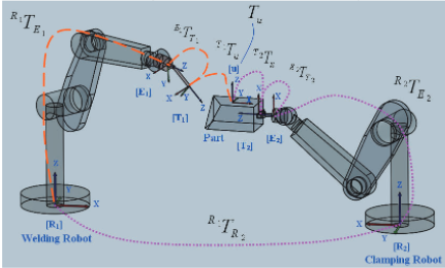
\includegraphics[width=9cm]{images/JointCoordinate2robs.png}
   \caption[Two Robot Coordinate System]
   {Two Robot Coordinate System \footnotemark[\value{footnote}]}  
\label{fig:img4}
\end{figure}
In non master/slave mode the pose of an object is set based on time. The mathematical description of the seams to be welded are specified based on which the transformations from robot 1 to work piece edge ${R1}^T_{E1} $ are calculated and similarly for robot 2 and work piece ${R2}^T_{E1}$. The seam to be welded is also described mathematically in this approach similar to \cite{7}. The kinematic scheme of the two robots and the work piece is illustrated with the following equation \eqref{eq15}.

\begin{equation}
\label{eq15}
{_{E_{1}}^{R_{1}}\textrm{T}} *{_{T_{1}}^{E_{1}}\textrm{T}} *{_{u}^{T_{1}}\textrm{T}} = {_{R_{2}}^{R_{1}}\textrm{T}} *{_{E_{2}}^{R_{2}}\textrm{T}}*{_{T_{2}}^{E_{2}}\textrm{T}} *{_{u}^{T_{2}}\textrm{T}} = _{u}T
\end{equation}

In \eqref{eq15} ${_{E_{i}}^{R_{i}}\textrm{T}} $ indicates the transformation matrix of end effector of robot i with respect to base of robot i. \\
the term ${_{T_{i}}^{E_{i}}\textrm{T}} $ indicates the transformation matrix of tool tip of robot i with respect to end effector i. \\ 
the term ${_{R_{2}}^{R_{1}}\textrm{T}} $ indicates the transformation matrix of robot 2 with respect to robot 1. \\ 
the term ${_{u}^{T_{i}}\textrm{T}} $ indicates the transformation matrix of work piece edge u with respect to tool tip i.\\
The authors conclude in the results section that using this approach will give the user greater capabilities to weld complex edges as the two 6 dof manipulators are more than enough to address collision avoidance and reachability issues. However a drawback of this method to be kept in mind is that for each edge to be welded, (no matter how complex it is geometrically) accurate mathematical description needs to be formulated. This greatly reduces flexibility for welding new edges. 


\subsection{Welding as an Optimization Problem}
Current industrial are mostly pre-programmed and used to perform repetitive tasks. Hence they are unsuitable to be used in small and medium enterprises, where the welding tasks are flexible as the work piece itself may vary from task to task. It goes without saying that the welding process not only needs to be flexible but also needs to adapt based on the shape of the work piece to be welded. Furthermore it needs to finish the welding task in minimum time while consuming minimum resources (power, weld material) as well as ensuring optimal weld quality. This suggests that welding can be treated as an optimization problem with time to weld and motion cost as the cost functions; which are to be minimized. Two major approaches usually taken in this regard are 
\begin{enumerate}
\item Specify the optimization criteria as extra constraints and generate path plans subject to these additional constraints
\item Adding certain heuristics to existing planning algorithms to generate more optimized plans.
\end{enumerate}
The approaches are elaborated in the following sub sections.
\subsubsection{Welding Process Parameters Optimization}
In \cite{9}(weld quality assessment based on arc sensing), the authors propose a real time analysis of signals in frequency domain to give feedback to the robot controller in real time.The authors record current and voltage consumed during the welding process and then apply power spectral density and time frequency analysis methods to analyze them. The authors use Short Time Fourier Transform(SFTT) to analyze each frequency component of the recorded signals. The authors conducted extensive experiments and came to the conclusion that the developed system performs reasonably well, and is able to optimize the task and take into account any possible defects, however the performance is subject to constrains of accuracy of real time data collection and monitoring. Even though this method is computationally simple and easy to implement, but since the authors only test this method on geometrically simple welding tasks e.g. straight lines, it is difficult to truly gauge the performance of this optimization method. A similar method of regulating the current supplied to the weld tool tip to optimize the weld quality has been presented in \cite{10}(Effect of weld parameters on weld quality in sheet to tube..). The authors propose a method in which the current is varied with each point on the weld trajectory and the tensile strength of the weld spot is measured. From the experiments conducted the authors concluded that that as welding progresses the temperature of the weld surface increases and it results in reduced tensile strength of the weld surface. Also continuously increasing the current led to improvement in welding upto a certain level but beyond a certain point the effect of current became detrimental to the weld quality. Even though this paper lacks a model based approach, it provides key insight about the relationship of various parameters to weld quality.
In \cite{10}(Time optimal trajectory planning for a 6R..) the authors use a genetic algorithm based approach to optimize the trajectory generated for the robot. The authors first model the dynamics of the robot using standard kinematics and inverse kinematic equations. While applying the genetic algorithm, the following steps are taken
\begin{enumerate}
\item Fitness function: transforming the constraint equations into fitness functions
\item Determining the generic operators: since the authors use an adaptive genetic algorithm the crossover and mutation parameter change with each step so as to ensure the algorithm neither converges pre maturely nor it becomes too wide which leads to non convergence.
\item The initial, final and the middle points are determined through which the robot is expected to travel
\item Apply recursive trajectory planning for each segment
\item Apply adaptive genetic algorithm to compute the fitness function and produce the new generation.
\item Repeat until desired solution with value lesser than desired maximum cost is obtained
\item The final optimal trajectory for each section of the path is obtained along with the time required to traverse it.
\end{enumerate} 
The paper lack concrete experimentation and proper results of the experimentation has not been provide which makes it difficult to assess the actual performance of the adaptive genetic algorithm based approach. 
In \cite{12}(Simulation Planning of Robot Welding) the authors propose a method of process optimization in the following areas of a welding operation; robot location, weld gun selection and motion controlling.            
For weld gun selection the authors measure the suitability of the weld gun based on the size and shape of the work piece and the work space available as well as the reach-ability of the weld head in that particular work space. The selection can be made from x type and c type weld heads. Next the authors describe the positioning of the robot manipulator, tool tip, work piece object and other components of the weld cell, in the welding work space. The following diagram \ref{fig:img6} describes in brief the hierarchical structure followed in order to define the process.
\begin{figure}[htbp] %  figure placement: here, top, bottom, or page
 \centering
   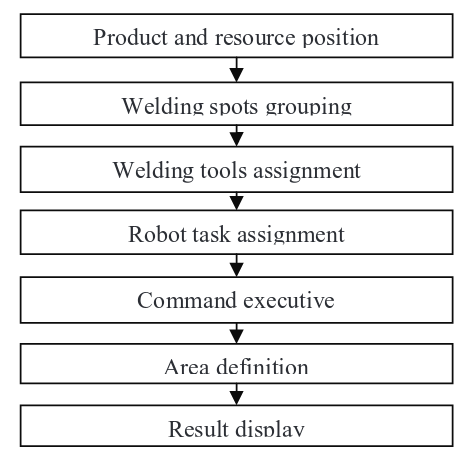
\includegraphics[width=9cm]{images/robotlocproc.png}
   \caption[Robot Location Model]
   {Robot Location Model \footnotemark[\value{footnote}]}  
\label{fig:img6}
\end{figure}
The product and resource position describe the positioning of the robots, work piece object, tool center point(TCP) and the weld gun. In welding spots grouping, the definition for the seam to be welded are defined. The tool to be assigned based on the work space is determined in welding tool assignment section. After the selection of the weld tool head and the work piece seam, the robot task is assigned. The task section contains definition of the work space in which the plan for the robot is to be generated usually in Cartesian coordinate system. It contains description of the weld seam and any collision objects, if present. After the plan is generated, it is executed on the robot inside the area definition. Finally the results of the planned path is displayed. \\ In the optimization section, the authors break down the final trajectory of the robot in basic motions -  such as joint, linear, circle and slew - which can be followed by the robot easily. After this step, the planned path is crash tested and modified accordingly. This paper lays the ground work for a hierarchical welding process model. However a lack of concrete implementation and subsequent testing leaves an open question about the feasibility of the described model. Few more papers on this topic have been evaluated in the later sections.

\subsubsection{Parameter Optimization of Motion Planning Algorithms}
In this section we will delve into work that focuses on optimizing the actual planner in order to generate optimal paths. In \cite{11}(HGRRT*) the authors propose an optimization based on user given input. The state cost definition is based on potential field framework. The planning algorithm minimizes motion cost by taking path segments with minimum cost while also optimizing the time required to generate the plan. In this approach the authors use a potential field function to guide the sampler of the RRT* algorithm to sample in used desired spaces. The state cost function is calculated using the following equation \eqref{11}
\begin{equation}
\label{16}
c(s) = \sum_{i} max(-\lambda_{i},0 ) + \lambda_{i}e^{\alpha_{i}d_{i}(s)^2} \epsilon (0,\sum_{i}|\lambda_{i}|]
\end{equation}
with $\lambda_{i} \epsilon \Re$ and $d_{i}(s)$ is the distance between work space and robot's reference point. The motion cost for the entire planned path is calculated based on the sequence of states with state costs with the following equation \eqref{16}
\begin{equation}
\label{17}
c(P) = \sum_{i=1}^{n-1}c(s_{i},s_{i+1})
\end{equation}
The proposed algorithm is illustrated as follows
\begin{itemize}
\item Sample: Random sample is generated in configuration space with probability 1 - $P_{goal}$ and for the goal state the probability is $P_{goal}$
\item Returns the k nearest neighbors of a state q. The value of k depends on dimension of configuration space.
\item Returns the path connecting initial state $q_{init}$ and goal state $q_{goal}$ composed by edges of the planning tree.
\item Collision free (q1, q2): Checks for collision between states q1 and q2 and returns the result.
\item Nearest: the closest node to q is returned. 
\item Cost: Returns the state cost of q
\item EdgeCost(q1, q2): Returns the cost between state q1 and q2
\end{itemize}
The authors conducted experiments and compared the results with TRRT algorithm. From the results it was concluded that the TRRT takes lesser time to find the solution path, however HGRRT* found shorter and more cost efficient paths. 
\subsection{Robotic Welding Architecture and Planning in Abstract Space}
\subsubsection{Product, Process and Resource Model}
\subsubsection{Implementation Platform Architecture}
jjdjdjd
